\section{Introduction}
\label{sec:intrp}

In the early 1980's, the British Broadcasting Corporation (BBC)
introduced a whole generation of educators and students in the United Kingdon (UK)
to computing through the {\em BBC Computer Literacy Project}, which featured the BBC Micro,
a 6502-based personal computer designed and produced by Acorn Computers Ltd. (referred
to at times as the ``British Apple'').  The project was very sucessful:
more than 80\% of UK classrooms had a BBC Micro and many of today's
computing professionals from the UK first encountered computing through
the BBC Micro[REF].

Fast forward to 2015: the BBC sought to again inspire a new
generation get creative with coding, programming and digital technology
through its {\em Make It Digital} initiative, as well as to support the UK's mandate to
teach computer science concepts at all grade levels.~\cite{PeytonJones2013ICFP}

As part of this effort, the BBC introduced the micro:bit (see
Figure~\ref{fig:microbit}),
a small programmable and embeddable computer designed,
developed and deployed by the BBC and partners (including ARM, Microsoft
and Lancaster University) to approximately 800,000 UK middle school students
in 2015-2016. Harkening back to its work with the BBC Micro,
the BBC described the micro:bit as its ``most ambitious education initiative in 30 years,
with an ambition to inspire digital creativity and
develop a new generation of tech pioneers.''~\cite{BBCwebsite}

By embracing a simplified constructionist~\cite{Papert} approach to computing education, the micro:bit has moved from
a local educational experiment in the UK to a global phenomenon, now present in over 37 countries.
Driving the worldwide expansion is
the Micro:bit Educational Foundation (\url{www.microbit.org}),
a non-profit organization
established in September 2016, with the support of its founding partners.~\footnote{ARM,
Amazon, BBC, British Council, IET, Lancaster University, Microsoft,
Nominet, and Samsung.}

We describe the motivation for and design of the BBC micro:bit (Section~\ref{sec:microbit}),
and present a sampling of micro:bit projects that
show off the device's capabilities (Section~\ref{sec:projects}). We then detail
the rollout of the micro:bit in the UK and around the world, via the partner-based approach
taken by both the BBC and the Foundation (Section~\ref{sec:mef}).

We draw from two full years of
full deployment of the micro:bit in the UK, as well as deployments
in Europe, the Americas, and Asia.  There are approximately
two million micro:bits now in the market and many hardware,
content, and education partners participating.

%Purpose
%- what is the micro:bit?
% http://www.bbc.co.uk/programmes/articles/4hVG2Br1W1LKCmw8nSm9WnQ/the-bbc-micro-bit


% reference the competition and show what's different (hardware)
% https://barrettsprojects.wordpress.com/2012/09/15/tap-and-double-tap/

\begin{figure}
  \begin{tabular}{cc}
    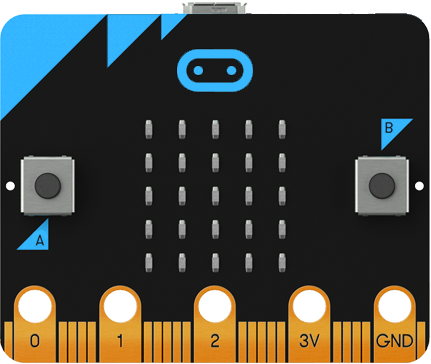
\includegraphics[width=1.5in]{images/microbit-front.png} &
    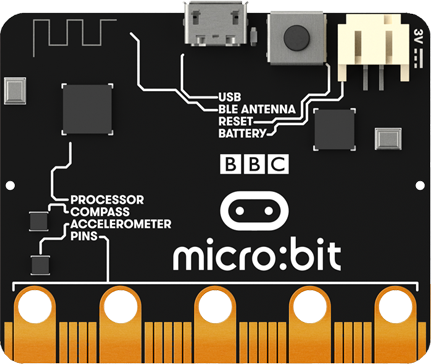
\includegraphics[width=1.5in]{images/microbit-back.png} \\
    (a) & (b)
  \end{tabular}
  \caption{\label{fig:microbit}The micro:bit: (a) front, with two buttons,
    5x5 LED display, and edge connector (bottom); (b) back, with processor, accelerometer, compass, Bluetooth, USB and battery ports.}
  \end{figure}

 